\lecture{9}{2025-11-24}{}

\section{Multi-tape Turing machines}

\subsection{Variants of Turing machines}

\begin{eg}
    The transition function may be defined as
    \[
        \delta: Q \times \Gamma \to Q \times \Gamma \times \{L, R, S\}
    \]
\end{eg}

\begin{notation}
    $S$ stands for ``stay'', meaning the head does not move.
\end{notation}

This kind of Turing machine can be simulated by a standard Turing machine.
\begin{align*}
    q_1, a \to q_2, b, S \ \     \equiv \
    &q_1, a \to q_{\text{temp}}, b, R \\
    &q_{\text{temp}}, \gamma \to q_2, \gamma, L \quad \forall \gamma \in \Gamma
\end{align*}

\subsection{Multi-tape Turing machines}

In this variant, there are multiple tapes, each with its own head.
\begin{itemize}
    \item Input: In the first tape.
    \item Other tapes: Blank initially.
    \item \begin{definition}[Multi-tape Turing machine]
        Transition function:
        \[
            \delta: Q \times \Gamma^k \to Q \times \Gamma^k \times \{L, R, S\}^k \quad \text{(for $k$ tapes)}
        \]
    \end{definition} 
\end{itemize}

\begin{eg}
    Given $w = 0^{2n}, \ n \geq 1 \ \Rightarrow$ Generate $ww$.
\end{eg}

\begin{idea}
    We have the following simulation:
    \begin{itemize}
        \item Copy $w$ into the second tape.
        \item Check if $|w|$ is even.
        \item copy $w$ from the second tape to the first tape (append).
    \end{itemize}
\end{idea}

\begin{figure}[H]
    \centering
    \begin{tikzpicture}[node distance=3cm, ->, >=Stealth, on grid, auto]
      \node[state,initial below] (q_0) {$q_0$};
      \node[state,right of=q_0,xshift=-0.3cm] (q_1) {$q_1$};
      \node[state,right of=q_1,xshift=-0.3cm] (q_2) {$q_2$};
      \node[state,right of=q_2,xshift=-0.5cm] (q_3) {$q_3$};
      \node[state,right of=q_3,xshift=-0.3cm] (q_4) {$q_4$};
      \node[state,below of=q_4,yshift=0.5cm] (q_a) {$q_a$};
      \path (q_0) edge[above] node{
        \begin{tabular}{l}
          $0 \rightarrow$ R\\
          $\sqcup \rightarrow$ R      
        \end{tabular}
      } (q_1);
      \path (q_1) edge[loop below] node{
        \begin{tabular}{l}
          $0 \rightarrow$ R\\
          $\sqcup \rightarrow 0,$ R      
        \end{tabular}
      } (q_1);
      \path (q_1) edge[above] node{
        \begin{tabular}{l}
          $\sqcup \rightarrow$ L\\
          $\sqcup \rightarrow$ L      
        \end{tabular}
        } (q_2);
      \path (q_2) edge[above, bend left] node{
        \begin{tabular}{l}
          $0 \rightarrow$ R\\
          $0 \rightarrow$ L
        \end{tabular}
        } (q_3);
      \path (q_3) edge[below, bend left] node{
        \begin{tabular}{l}
          $\sqcup \rightarrow $ L\\
          $0 \rightarrow$ L      
        \end{tabular}
        } (q_2);
      \path (q_3) edge[above] node{
        \begin{tabular}{l}
          $\sqcup \rightarrow$ 0, R\\
          $\sqcup \rightarrow$ 0, R      
        \end{tabular}
        } (q_4);
      \path (q_4) edge[loop above] node{
        \begin{tabular}{l}
          $\sqcup \rightarrow$ 0, R\\
          $0 \rightarrow$ R      
        \end{tabular}
        } (q_4);
      \path (q_4) edge[left] node{
        \begin{tabular}{l}
          $\sqcup \rightarrow$ R\\
          $\sqcup \rightarrow$ R
        \end{tabular}
        } (q_a);
    \end{tikzpicture}
    \caption{Multi-tape Turing machine to compute $ww$ from $w = 0^{2n}$}
\end{figure}

\newpage

For the simulation details,
\begin{itemize}
    \item $q_0 \to q_1$: Use $\sqcup$ to indicate the beginning of the second tape.
    \item loop in $q_1$: Copy $w$ from the first tape to the second tape.
    \item $q_2 \to q_3 \to q_2$: 
    \begin{enumerate}[label=$\arabic*^\circ$]
        \item Check if length of $w$ is even.
        \item Head of the first tape zig-zag between last $0$ and then $\sqcup$ after.
        \item Head of the second tape moves to the beginning.
    \end{enumerate}
    \begin{remark}
        If length of $w$ is even, we will at $q_3$ when reaching the beginning of the second tape.
    \end{remark}
    \item $q_4$: copy $w$ from the second tape to the first tape (append).
\end{itemize}

Below is the illustration of the simulation $0000$:
\begin{center}
    
    {
    \setlength{\tabcolsep}{5pt}      
    \renewcommand{\arraystretch}{1.7}  
    \begin{tabular}{@{}llll}
    $ q_0
    \begin{smallmatrix}
      0 &0 & 0 & 0 \\
      \sqcup & \sqcup & \sqcup & \sqcup
    \end{smallmatrix}
    $
    &
    $
    \begin{smallmatrix}
      0 \\
      \sqcup 
    \end{smallmatrix}
    q_1
    \begin{smallmatrix}
      0 & 0 & 0 \\
      \sqcup & \sqcup & \sqcup
    \end{smallmatrix}
    $
    &           
    $\cdots
    $
    &
    $
    \begin{smallmatrix}
      0 & 0 & 0 & 0\\
      \sqcup & 0  & 0 & 0
    \end{smallmatrix}
    q_1
    \begin{smallmatrix}
      \sqcup\\
      \sqcup 
    \end{smallmatrix}
    $
    \\
    $
    \begin{smallmatrix}
      0 & 0 & 0 \\
      \sqcup & 0  & 0 
    \end{smallmatrix}
    q_2
    \begin{smallmatrix}
      0\\
      0
    \end{smallmatrix}
    $
    &
    $
    \begin{smallmatrix}
      0 & 0 & & 0 & 0 & q_3\\
      \sqcup & 0 & q_3 & 0 & 0 &
    \end{smallmatrix}
    $
    & 
    $
    \begin{smallmatrix}
      0 & & 0 & 0 & q_2 & 0\\
      \sqcup & q_2 & 0 & 0 &&  0 
    \end{smallmatrix}
    $
    &
    $
    \begin{smallmatrix}
      & 0 & 0 & 0 & 0 & q_3\\
      q_3 & \sqcup & 0 & 0 & 0 
    \end{smallmatrix}
    $
    \\
    $
    \begin{smallmatrix}
       0 & & 0 & 0 & 0 & 0 & q_4\\
      0 & q_4 & 0 & 0 & 0 & \sqcup
    \end{smallmatrix}
    $
    & 
    $\cdots$
    &
    $
    \begin{smallmatrix}
       0 & 0 & 0 & 0 & 0 & 0 & 0 & 0 & q_4\\
      0 &  0 & 0 & 0 & q_4 &&&&
    \end{smallmatrix}
    $
    &
    % $
    % \begin{smallmatrix}
    %    0 & 0 & 0 & 0 & 0 & 0 & 0 & 0 & \sqcup & q_a\\
    %   0 &  0 & 0 & 0 & \sqcup & q_a &&&
    % \end{smallmatrix}
    % $
    \end{tabular}
    \renewcommand{\arraystretch}{1}
    }
\end{center}

Below is the illustration of the simulation $000$:
\begin{center}
    \renewcommand{\arraystretch}{1.7}  
  \begin{tabular}{llll}
$ q_0
\begin{smallmatrix}
  0 &0 & 0 \\
  \sqcup & \sqcup & \sqcup 
\end{smallmatrix}
$
&
$
\begin{smallmatrix}
  0 \\
  \sqcup 
\end{smallmatrix}
q_1
\begin{smallmatrix}
  0 & 0  \\
  \sqcup & \sqcup 
\end{smallmatrix}
$
&           
$\cdots
$
&
$
\begin{smallmatrix}
  0 & 0 & 0 \\
  \sqcup & 0  & 0 
\end{smallmatrix}
q_1
\begin{smallmatrix}
  \sqcup\\
  \sqcup 
\end{smallmatrix}
$
\\
$
\begin{smallmatrix}
  0 & 0  \\
  \sqcup  & 0 
\end{smallmatrix}
q_2
\begin{smallmatrix}
  0\\
  0
\end{smallmatrix}
$
&
$
\begin{smallmatrix}
  0 & & 0 & 0 & q_3\\
  \sqcup & q_3 & 0 & 0 &
\end{smallmatrix}
$
& 
$
\begin{smallmatrix}
  & 0  &  0 & q_2 & 0\\
  q_2 & \sqcup & 0 &  & 0 
\end{smallmatrix}
$
&
\end{tabular}
\renewcommand{\arraystretch}{1}
\end{center}

\begin{note}
    Due to the properties of ``deterministic'',
    \[
        \delta(q_0, 0, 0),\ \delta(q_0, 0, \sqcup)\  \delta(q_0, \sqcup, 0),\ \delta(q_0, \sqcup, \sqcup)
    \] 
    those not specified transitions go to $q_r$.
\end{note}

\subsection{Multi-tape TM $\equiv$ Single-tape TM}

\begin{figure}[H]
    \centering
    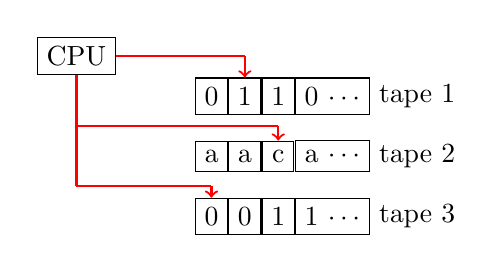
\begin{tikzpicture}[ampersand replacement=\&]
    \matrix 
    {
    \node[draw](0) {CPU}; \& [1cm]  \& \node(1){} ; \&\&\& \\
    \& \node[draw]{0}; \& \node[draw](a){1}; \& \node[draw]{1}; \& \node[draw]{0 $\cdots$};  \& \node{tape 1};\\
    \node(2){} ; \&  \&  \& \node(21){} ; \&\& \\  
    \& \node[draw]{a}; \& \node[draw]{a}; \& \node[draw](b){c}; \& \node[draw]{a $\cdots$}; \&  \node{tape 2}; \\
    \node(3){} ; \& \node(31){} ; \&  \&  \&\& \\
    \& \node[draw](c){0}; \& \node[draw]{0}; \& \node[draw]{1}; \& \node[draw]{1 $\cdots$}; \&  \node{tape 3}; \\
    };

    \draw [-,red,thick] (0) -- (1.center) ;
    \draw [->,red,thick] (1.center) -- (a) ;
    \draw [-,red,thick] (0) -- (2.center) ;
    \draw [-,red,thick] (2.center) -- (21.center) ;
    \draw [->,red,thick] (21.center) -- (b) ;
    \draw [-,red,thick] (0) -- (3.center) ;
    \draw [-,red,thick] (3.center) -- (31.center) ;
    \draw [->,red,thick] (31.center) -- (c) ;
    \end{tikzpicture}
    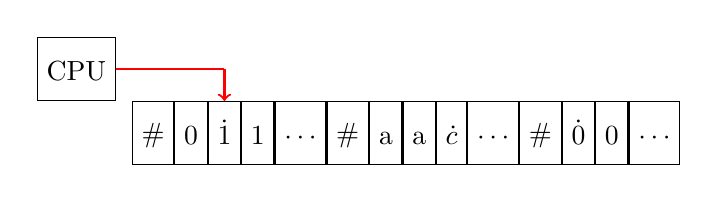
\begin{tikzpicture}[ampersand replacement=\&]
    \matrix[nodes={minimum height=8mm,text height=0.3cm}] 
    {
    \node[draw](0) {CPU}; \& [0.2cm] \& \& \node(1){} ; \& \&\&\& \&\&\& \&\&\& \\
    \& \node[draw]{\#};  \& \node[draw]{0}; \& \node[draw](a){$\dot{1}$}; \& \node[draw]{1}; \& \node[draw]{$\cdots$};
    \& \node[draw]{\#};  \& \node[draw]{a}; \& \node[draw]{a}; \& \node[draw]{$\dot{\text{c}}$}; \& \node[draw]{$\cdots$}; 
    \& \node[draw]{\#};  \& \node[draw](c){$\dot{0}$}; \& \node[draw]{0}; \& \node[draw]{$\cdots$}; \\
    };

    \draw [-,red,thick] (0) -- (1.center) ;
    \draw [->,red,thick] (1.center) -- (a) ;
    \end{tikzpicture}
    \caption{Simulation of multi-tape Turing machine by single-tape Turing machine}
\end{figure}

\begin{itemize}
    \item $\#$ can be used to separate different tapes.
    \item $\dot{c}$ can be used to indicate the head position of each tape.
    \item $\Gamma' = \{ \Gamma, \dot{\Gamma} \}$
\end{itemize}

\newpage

\begin{eg}
    Right shifting a sequece $w$.
\end{eg}

\begin{figure}[H]
    \centering
    \begin{tikzpicture}[node distance=2.5cm, ->, >=Stealth, on grid, auto]
      \node[state] (q_s) {$q_s$};
      \node[state,above right of=q_s,xshift=1.7cm] (q_0) {$q_0$};
      \node[state,below right of=q_s,xshift=1.7cm] (q_1) {$q_1$};
      \node[state,below right of=q_0,xshift=1.7cm] (q_a) {$q_a$};    
      \path (q_s) edge[above] node{
           $0 \rightarrow \sqcup,$ R
         } (q_0);
      \path (q_s) edge[below] node{
           $1 \rightarrow \sqcup,$ R
      } (q_1);
      \path (q_0) edge[bend right=15, left] node{
           $1 \rightarrow 0,$ R
         } (q_1);
      \path (q_0) edge[loop right] node{
           $0 \rightarrow $ R
      } (q_0);
      \path (q_1) edge[bend right=15, right] node{
           $0 \rightarrow 1,$ R
      } (q_0);
      \path (q_1) edge[loop right] node{
           $1 \rightarrow $ R
      } (q_1);
      \path (q_0) edge[above] node{
           $\sqcup \rightarrow 0$ 
      } (q_a);
      \path (q_1) edge[below] node{
           $\sqcup \rightarrow 1$ 
      } (q_a);
    \end{tikzpicture}
    \caption{Single-tape simulation Turing machine to right shift a sequence}
\end{figure}

\begin{note}
    Because $\Gamma$ is finite, the simulation must succeed by add state for each $\gamma \in \Gamma$.
\end{note}

\section{Nondeterministic Turing Machines}

\begin{definition}[Nondeterministic Turing machine]
    Transition function:
    \[
        \delta: Q \times \Gamma \to \mathcal{P}(Q \times \Gamma \times \{L, R\})
    \]
\end{definition}

In NTM, by definition $w$ is accepted if any branch
works, which means unless all branches are finite,
\[
    \text{NTM} \ \longrightarrow \ \text{accept or loop}
\]
Thus, NTM is an ``acceptor''.

\begin{eg}
    $A = \{ w \text{ contain } aab \}$
\end{eg}
\begin{figure}[H]
    \centering
    \begin{tikzpicture}[node distance=2.5cm, ->, >=Stealth, on grid, auto]
  \node[state,initial] (q_0) {$q_0$};
  \node[state,right of=q_0] (q_1) {$q_1$};
  \node[state,right of=q_1] (q_2) {$q_2$};
  \node[state,right of=q_2] (q_a) {$q_a$};
  \node[state,below right of=q_0,yshift=-0.5cm] (q_r) {$q_r$};
  \path (q_0) edge[loop above] node{
      $a, b \rightarrow a, b,$ R
    } (q_0);
  \path (q_0) edge[above] node{
      $a \rightarrow$ R
  } (q_1);
  \path (q_1) edge[above] node{
      $a \rightarrow$ R
  } (q_2);
  \path (q_2) edge[above] node{
      $b \rightarrow$ R
    } (q_a);
  \path (q_0) edge[left] node{
      $\sqcup \rightarrow$ R      
    } (q_r);
  \path (q_1) edge[right] node{
    \begin{tabular}{l}
      $b \rightarrow$ R\\
      $\sqcup \rightarrow$ R      
    \end{tabular}
    } (q_r);
  \path (q_2) edge[right, bend left] node{
    \begin{tabular}{l}
      $a \rightarrow$ R\\
      $\sqcup \rightarrow$ R      
    \end{tabular}
    } (q_r);
    \end{tikzpicture}
    \caption{Nondeterministic Turing machine to accept $A = \{ w \text{ contain } aab \}$}
\end{figure}
\begin{note}
    Determine where $aab$ starts nondeterministically.
\end{note}

\begin{eg}
    $L = \{ 0^n \mid n\text{-composite number} \}$
\end{eg}
\begin{itemize}
    \item Nondeterministically guess $p, q$, sequentially try from $2$ to $n-1$.
    \item Check if $n = p \times q$
\end{itemize}

\newpage

\subsection{NTM $\equiv$ TM}

A language is Turing-recognizable $\implies$ it is recognized by a NTM, due to TM being a special case of NTM. Proof done for $\Leftarrow$ direction. \\

For the other direction, we need to simulate NTM by TM. Like NFA we use a tree structure to represent the computation finite $\#$ branches. To traverse the tree, we can use BFS or DFS.
\begin{remark}
    BFS is preferred, because DFS may get stuck in an infinite branch.
\end{remark}

\begin{figure}[H]
    \centering
    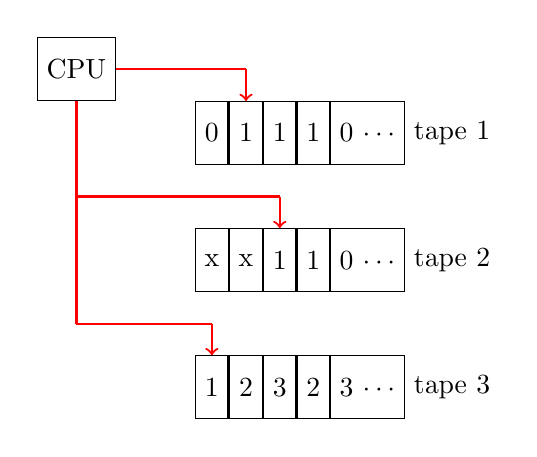
\begin{tikzpicture}[ampersand replacement=\&]
    \matrix[nodes={minimum height=8mm}]     
    {
    \node[draw](0) {CPU}; \& [1cm]  \& \node(1){} ; \&\&\& \& \\
    \& \node[draw]{0}; \& \node[draw](a){1}; \& \node[draw]{1}; \& \node[draw]{1};  \& \node[draw]{0 $\cdots$};  \& \node{tape 1};\\
    \node(2){} ; \&  \&  \& \node(21){} ; \&\& \&\\  
    \& \node[draw]{x}; \& \node[draw]{x}; \& \node[draw](b){1}; \& \node[draw]{1}; \& \node[draw]{0 $\cdots$}; \& \node{tape 2};  \\
    \node(3){} ; \& \node(31){} ; \&  \&\& \& \&\\
    \& \node[draw](c){1}; \& \node[draw]{2}; \& \node[draw]{3}; \& \node[draw]{2}; \& \node[draw]{3 $\cdots$}; \&  \node{tape 3}; \\
    };

    \draw [-,red,thick] (0) -- (1.center) ;
    \draw [->,red,thick] (1.center) -- (a) ;
    \draw [-,red,thick] (0) -- (2.center) ;
    \draw [-,red,thick] (2.center) -- (21.center) ;
    \draw [->,red,thick] (21.center) -- (b) ;
    \draw [-,red,thick] (0) -- (3.center) ;
    \draw [-,red,thick] (3.center) -- (31.center) ;
    \draw [->,red,thick] (31.center) -- (c) ;
    \end{tikzpicture}
    \caption{Simulation of NTM by TM using multi-tape Turing machine}
\end{figure}

\begin{itemize}
    \item Tape 1: Store the input, never alter.
    \item Tape 2: Simulate the current branch up to certain layer by copying Tape 1.
    \item Tape 3: Store the path to a node.
    \begin{definition}
        Suppose max $\#$ branches is $3$ at each node. If the content of the 3rd tape is \(
            2 3 1
        \) that means \[
            \text{root} \to \text{2nd child} \to \text{3rd child} \to \text{1st child}
        \]
    \end{definition}
\end{itemize}

Hence, NTM can be simulated by 3-tape TM, and we have shown that multi-tape TM can be simulated by single-tape TM. Thus, NTM $\equiv$ TM. \hfill \qed

\begin{corollary}
    NTM is a decider if all branches halt on all inputs.
    \[
        \text{Language decidable} \iff \text{some NTM decides it}
    \]
\end{corollary}
\begin{proof}
    We separate into two directions.
    \begin{itemize}
        \item[$\Rightarrow$] One TM decides it and a TM is an NTM. This TM halts on all inputs (one branch)
        \item[$\Leftarrow$] Now NTM terminates on all branches. We can construct a TM to decide the language
        \begin{itemize}
            \item each branch is finite every input halts $\exists$ a finite max length.
            \item $\#$ branches finite. The tree to process this input is finite.
            \item Thus the three-tape TM used earlier can accept/reject the input in a finite number of steps.
        \end{itemize}
    \end{itemize}
\end{proof}

\newpage

\section{Hilbert's problems}

Informally, an algorithm is a collection of instructions. Not until 1900 did Hilbert propose 23 unsolved problems in mathematics. The 10th problem is: 
\begin{quote}
    \textit{Is there a general method to determine whether a given polynomial equation with integer coefficients has an integer solution?}
\end{quote}
Hilbert didn't use the word ``algorithm'' but ``general method''. However, Hilbert explicitly asked the algorithm be ``devises''.

\subsection{Church-Turing thesis}

This is proposed by Alonzo Church and Alan Turing in 1936.

\begin{quote}
    \textit{Any function which would naturally be regarded as computable can be computed by a Turing machine.}
\end{quote}

\begin{definition}
    \[
        \text{Intuitive Algorithm} \equiv \text{Turing machine algorithm}
    \]
\end{definition}

\subsection{Hilbert's 10th problem}

Using the Church-Turing thesis, we have a question:
\begin{exercise}
    Define \[
        D = \{ P \mid P: \text{polynomial with integer root} \}
    \]
    is $D$ decidable?
\end{exercise}

\vspace{1em}

We first simplify the problem to one variable case.
\[  
    D_1 = \{ P \mid P: \text{polynomial of $x$ with integer root} \}
\]
If we try all integers one by one, it may not halt if no integer root exists. Thus, $D_1$ is Turing-recognizable but not decidable. \\

However, it can be proved that roots of a 1-variable
polynomial is within the range
\[
    -M \leq x \leq M, \quad M = \pm k \frac{\max |c_i|}{|c_1|}
\]
where 
\begin{itemize}
    \item $k$: $\#$ of terms
    \item $c_i$: coefficients of the polynomial
    \item $c_1$: leading coefficient
\end{itemize}

For instance, for \(4x^3 - 2x^2 + x - 7\), we have
\[
    M = \pm 4 \cdot \frac{7}{4} = \pm 7
\]

\newpage

The multi-variable case is much more complicated. In 1970, Matiyasevich proved that no such algorithm exists. Thus, we have the conclusion:
\begin{theorem}[Matiyasevich, 1970]
    $D$ is not decidable.
\end{theorem}

\subsection{Description of Turing machines}
A Turing machine can be describe in 3 levels:
\begin{itemize}
    \item \textbf{High-level description}: Describe the operations of the Turing machine without manage the tape and head.
    \item \textbf{Implementation-level description}: Describe how the Turing machine move the head.
    \item \textbf{Formal description}: Specify the states, input alphabet, tape alphabet, transition function, start state, accept state, and reject states of the Turing machine.
\end{itemize}

\begin{eg}
    Describe a Turing machine that decides the language 
    \[
        A = \{ \langle G \rangle \mid G: \text{ a connected undirected graph} \}
    \]
\end{eg}

\begin{itemize}
    \item \textbf{High-level description}: We separate into three steps.
    \begin{enumerate}[label=$\arabic*^\circ$]
        \item Mark node in $G$.
        \item Repeat until no new nodes marked:
        \begin{itemize}
            \item For each node in $G$, if it is marked, mark all its neighbors.
        \end{itemize}
        \item If all nodes marked: accept, otherwise: reject.
    \end{enumerate}
    \item \textbf{Implementation-level description}:
    \[
        \langle  G\rangle=(1,2,3,4)((1,2),(2,3),(3,1),(1,4))
    \] is the input format.
    \begin{figure}[H]
        \centering
            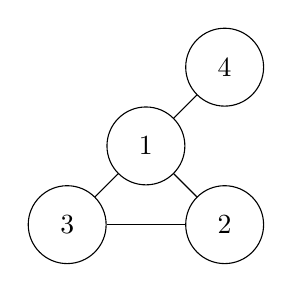
\begin{tikzpicture}[inner sep=2.5mm]      
            \path (0,0) node (3) [shape=circle,draw] {3}
            ( 2,0) node (2) [shape=circle,draw] {2}
            ( 2,2) node (4) [shape=circle,draw] {4}
            ( 1,1) node (1) [shape=circle,draw] {1};
            \draw [-] (1) -- (2);
            \draw [-] (2) -- (3);
            \draw [-] (1) -- (3);
            \draw [-] (1) -- (4);
            \end{tikzpicture}
        \caption{Graph representation on tape}
    \end{figure}
    \begin{itemize}
        \item The first step is to check if the input is in the correct format.
        \item In the first step we begin with seeing if the first part of the input $\langle G \rangle$ includes distinct numbers (as node IDs should be different)
        \item This is similar to an example before.
        \[
            \{ \# x_1 \# x_2 \# \cdots x_n \# \mid  x_i \in \{0,1\}^*, x_i \neq x_j \}
        \]
        \item Then we can talk about how the head is moved.
\end{itemize}